% vim: tw=78 ai sw=2 spell spelllang=en

\documentclass[xcolor=dvipsnames]{beamer}

\let\Oldemph\emph
\renewcommand{\emph}[1]{\textcolor{blue}{\Oldemph{#1}}}
\newcommand{\heading}[1]{\textbf{\textcolor{BurntOrange}{#1}}}

% Copyright 2004 by Till Tantau <tantau@users.sourceforge.net>.
%
% In principle, this file can be redistributed and/or modified under
% the terms of the GNU Public License, version 2.
%
% However, this file is supposed to be a template to be modified
% for your own needs. For this reason, if you use this file as a
% template and not specifically distribute it as part of a another
% package/program, I grant the extra permission to freely copy and
% modify this file as you see fit and even to delete this copyright
% notice. 


\mode<presentation>
{
%  \usetheme{Warsaw}
\usetheme{Madrid}
}

\setbeamertemplate{navigation symbols}{}

\usepackage[utf8]{inputenc}
\usepackage{times}
\usepackage[T1]{fontenc}

\usepackage{graphicx}
\usepackage[final]{listings}
\usepackage{multirow}

\lstset{tabsize=2,numbers=none,showstringspaces=false,breaklines=true,
	breakatwhitespace=true,escapeinside={(*@}{@*)},
	basicstyle=\scriptsize,keywordstyle=\bfseries\color{OliveGreen},
	commentstyle=\color{blue}}

\title{\textsc{Stanse}}

\subtitle{Bug-finding Framework for C Programs}

\author[Obdrzalek, Slaby, Trtik]{Jan~Obdrzalek, \emph{Jiri~Slaby},
Marek~Trtik\\ \hskip 1.5em \small{\textit{[Yiri Sla-be]}}}

\institute[FI MU]{ITI, Faculty of Informatics \\ Masaryk University
\\ Czech Republic}

\date{Oct 16 2011, Lednice}

\subject{Theoretical Computer Science}
% This is only inserted into the PDF information catalog. Can be left
% out. 



% If you have a file called "university-logo-filename.xxx", where xxx
% is a graphic format that can be processed by latex or pdflatex,
% resp., then you can add a logo as follows:

% \pgfdeclareimage[height=0.5cm]{university-logo}{university-logo-filename}
% \logo{\pgfuseimage{university-logo}}



% Delete this, if you do not want the table of contents to pop up at
% the beginning of each subsection:
% \AtBeginSubsection[]
% {
%   \begin{frame}<beamer>
%     \frametitle{Outline}
%     \tableofcontents[currentsection,currentsubsection]
%   \end{frame}
% }


% If you wish to uncover everything in a step-wise fashion, uncomment
% the following command: 

%\beamerdefaultoverlayspecification{<+->}

\begin{document}

\begin{frame}
  \titlepage
\end{frame}

%%%%%%%%%%%%%%%%%%%%%%%

\begin{frame}
  \frametitle{Presentation Outline}

  \begin{itemize}
  \item What is \textsc{Stanse}
  \item Current status
  \begin{itemize}
  \item What \textsc{Stanse} can do
  \item What algorithms/techniques \textsc{Stanse} comprises
  \end{itemize}
  \item Future work
  \end{itemize}

\end{frame}

\begin{frame}
  \frametitle{What is \textsc{Stanse}}

  \begin{center}
  
\includegraphics[height=5cm]{stanse}
  \end{center}

  \begin{itemize}
  \item Mainly a \emph{framework} for new static analysis techniques
  \pause
  \item But \emph{contains} some \emph{analyses} already
  \pause
  \item Developed at ITI FI, MU
  \end{itemize}

\end{frame}

\begin{frame}
  \frametitle{Why \textsc{Stanse}?}

  \heading{No framework for static analysis implementation}
  \begin{itemize}
  \item Free to use
  \item Easy to use
  \item For real C
  \item Providing enough of ``framework''
  \begin{itemize}
  \item E.g. inter-procedural analysis
  \end{itemize}
  \end{itemize}

\end{frame}

\begin{frame}
  \frametitle{\textsc{Stanse} as a Framework}
  
  \begin{itemize}
  \item Written in Java
  \begin{itemize}
  \item Ease of new techniques implementation
  \item Some drawbacks (see later)
  \end{itemize}

  \pause

  \item Provides various interfaces
  \begin{itemize}
  \item Requires a little work, everything needed is available
  \item Focus on the technique itself
  \end{itemize}
  \end{itemize}

\end{frame}

\begin{frame}
  \frametitle{Framework Status}

  \begin{itemize}
  \item \emph{Full ANSI C99 support}, including most GNU C extensions
    \begin{itemize}
    \item I.e. supports the Linux kernel
    \end{itemize}
  \item Easily extensible (modular design)
  \item Easy-to-use \emph{graphical interface}
  \item Intra- and inter-procedural analyses
  \item Batch + build system support (\textsc{make})
  \item Web interface for errors tracking
  \end{itemize}
\end{frame}

\begin{frame}[fragile]
  \frametitle{\textsc{Stanse} Parser}

  \begin{center}
  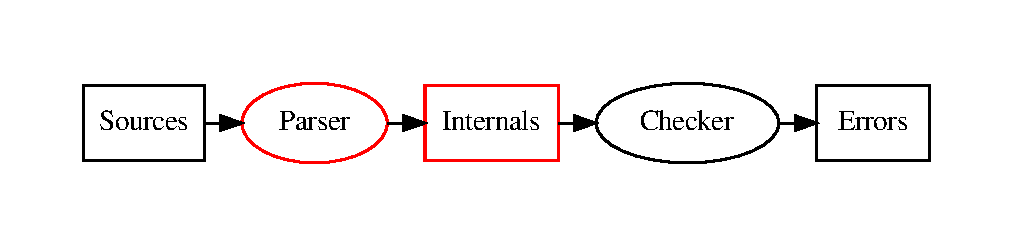
\includegraphics[trim=1.3cm 1.3cm 1.3cm 1.3cm,width=10cm]{level-parser}
  \end{center}

  \heading{Input: Source code} \\
  \heading{Output: Internal representation}

  \pause
  \medskip

  \heading{C parser}
  \begin{itemize}
  \item Preprocessor (modified GNU C)
  \item Machine-generated (\textsc{antlr})
  \begin{itemize}
  \item Relatively slow
  \end{itemize}
  \item Output
  \begin{itemize}
  \item Abstract Syntax Tree (AST) as XML
  \item Control Flow Graph (CFG)
  \item Call Graph (CG)
  \end{itemize}
  \end{itemize}

\end{frame}

\begin{frame}[fragile]
  \frametitle{Internal Structures Example}
  \begin{center}
  \begin{tabular}{|c|} \hline
  Source \\ \hline \hline
  \begin{lstlisting}[language=C]
if (cond)
  yes();
else
  no();
  \end{lstlisting} \\
  $\Downarrow$
  \end{tabular} \\
  \begin{tabular}{|c|c|} \hline
  AST (\texttt{$--$dump$-$xml}) & CFG (\texttt{$--$dump$-$cfg}) \\ \hline\hline
  \begin{lstlisting}[language=XML]
<ifElseStatement>
  <id>cond</id>         # cond
  <expressionStatement> # true
    <functionCall>
      <id>yes</id>
    </functionCall>
  </expressionStatement>
  <expressionStatement> # false
    <functionCall>
      <id>no</id>
    </functionCall>
  </expressionStatement>
</ifElseStatement>
  \end{lstlisting}
  & \parbox[c]{2.6cm}{\includegraphics[width=2.6cm]{cond}} \\ \hline
  \end{tabular}
  \end{center}

\end{frame}

\begin{frame}[fragile]
  \frametitle{\textsc{Stanse} Parser cont.}

  \begin{center}
  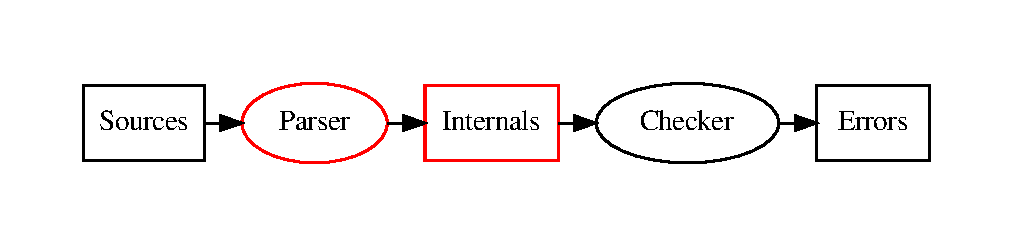
\includegraphics[trim=1.3cm 1.3cm 1.3cm 1.3cm,width=10cm]{level-parser}
  \end{center}

  \heading{Internal structures}
  \begin{itemize}
  \item Classes for walking through internals
  \item Support for large code bases
  \begin{itemize}
  \item Streaming
  \item Lazy parsing
  \end{itemize}
  \end{itemize}

\end{frame}

\begin{frame}
  \frametitle{Checkers}

  \begin{center}
  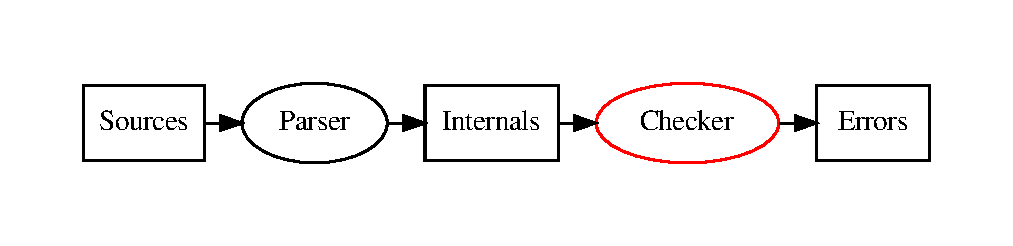
\includegraphics[trim=1.3cm 1.3cm 1.3cm 1.3cm,width=10cm]{level-checker}
  \end{center}

  \heading{Input: Internals} \\
  \heading{Output: Errors passed to the error management}

  \pause
  \medskip

  \begin{itemize}
  \item AutomatonChecker
  \item ThreadChecker
  \item LockChecker
  \item ReachabilityChecker
  \end{itemize}

\end{frame}

\begin{frame}
  \frametitle{AutomatonChecker}

  \begin{itemize}
  \item Finite automata for system behavior description
  \begin{itemize}
  \item Stems from \textsc{xgcc} (Stanford)
  \end{itemize}
  \end{itemize}
  \begin{center}
    \input{locking.pspdftex}
  \end{center}

  \pause

  \begin{itemize}
  \item Errors like imbalanced locking, NULL dereference, resource leaks
  \begin{itemize}
    \item Whatever can be described by FA, can be also checked
  \end{itemize}
  \end{itemize}
\end{frame}
  
\begin{frame}
  \frametitle{ThreadChecker}
  \begin{itemize}
  \item Finds and inspects threads behavior
  \item Watches locking and unlocking there
  \item Creates so-called Resource Allocation Graphs (RAG)
    \begin{itemize}
    \item For lock dependency tracking
    \end{itemize}
  \item Merges created RAGs and searches cycles
%  \item Finds non-trivial locking problems among threads
  \end{itemize}

  \begin{center}
  \begin{tabular}{ccccccc}
    \parbox{1cm}{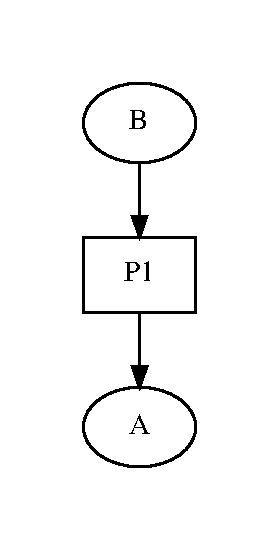
\includegraphics[trim=1.3cm 1.3cm 1.3cm 1.3cm,height=3.2cm]{RAG1}} & + &
    \parbox{1cm}{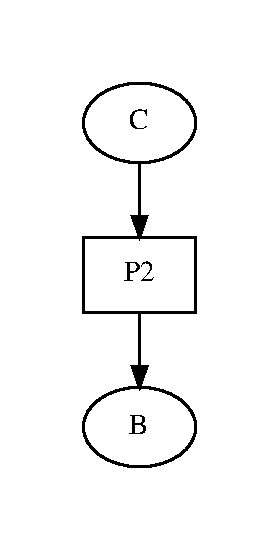
\includegraphics[trim=1.3cm 1.3cm 1.3cm 1.3cm,height=3.2cm]{RAG2}} & + &
    \parbox{1cm}{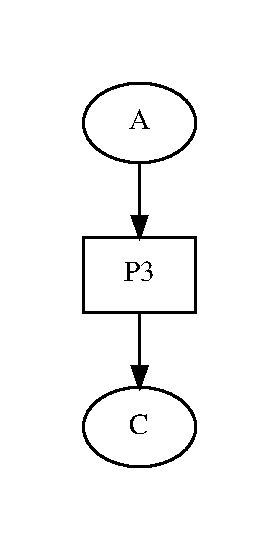
\includegraphics[trim=1.3cm 1.3cm 1.3cm 1.3cm,height=3.2cm]{RAG3}} & = &
    \parbox{3cm}{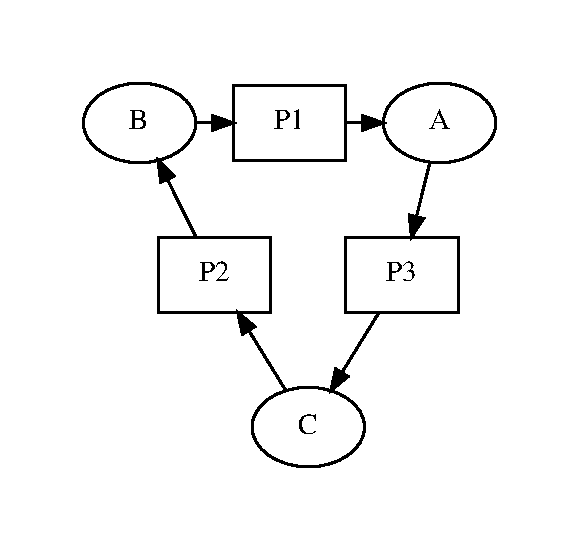
\includegraphics[trim=1.3cm 1.3cm 1.3cm 1.3cm,height=3.2cm]{RAG}}
  \end{tabular}
  \end{center}
\end{frame}
  
\begin{frame}[fragile]
  \frametitle{LockChecker}

  \begin{itemize}
  \item Statistical analysis (Engler)
  \item Tracks memory accesses
  \item Counts statistics, how many of them was with some lock held
  \item Ratio being at least 1:9 means a potential error
  \end{itemize}

  \begin{center}
  \begin{tabular}{|c|c|} \hline
  9$\times$ in code & 1$\times$ in code \\ \hline\hline
  \begin{lstlisting}[language=C]
lock(A);
glob_var = 1;
unlock(A);
  \end{lstlisting} &
  \begin{lstlisting}[language=C]
/* no lock */
glob_var = 5;
/* no unlock */
  \end{lstlisting} \\ \hline
  & \textcolor{red}{Potential error} \\ \hline
  \end{tabular}
  \end{center}

\end{frame}
  
\begin{frame}[fragile]
  \frametitle{ReachabilityChecker}
  \begin{itemize}
  \item Finds unreachable (dead) code
  \item Implemented in about 200 lines
  \item Serves as a demonstration for the framework
    \begin{itemize}
    \item In spite of that, it found some errors 
    \end{itemize}
  \end{itemize}

  \begin{center}
  \begin{tabular}{ccc}
  \begin{lstlisting}[language=C]
void fun(int error)
{
  // superfluous
  // semicolon
  //        |
  //        v
  if (error);
    return;
  // we won't
  // get here
  fun1();
  fun2();
}
  \end{lstlisting} & $\Rightarrow$ &
  \parbox[c]{5.5cm}{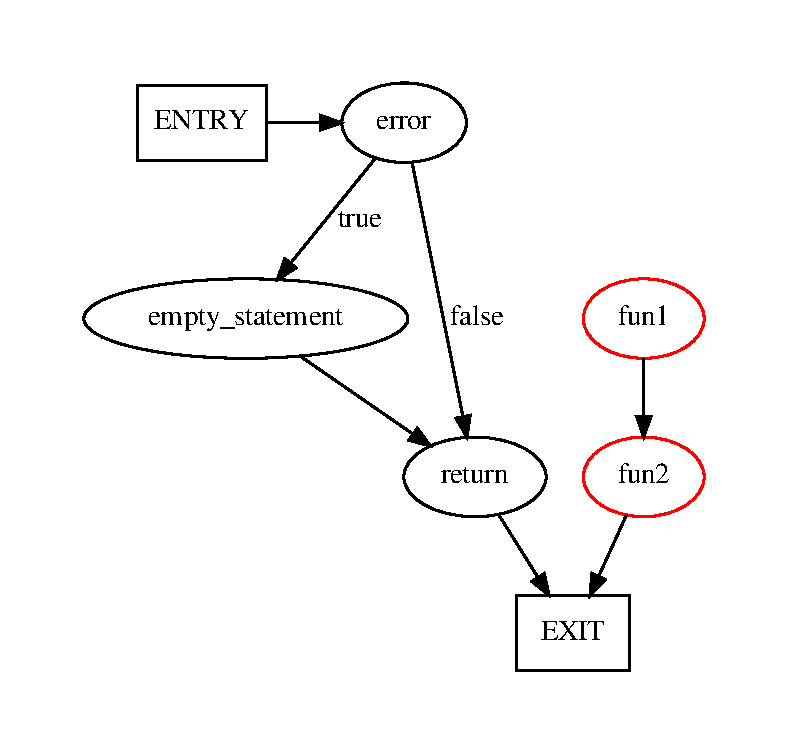
\includegraphics[trim=1.3cm 1.3cm 1.3cm 1.3cm,height=5cm]{dead}}
  \end{tabular}
  \end{center}

\end{frame}

\begin{frame}
  \frametitle{Configuration}

  \begin{center}
  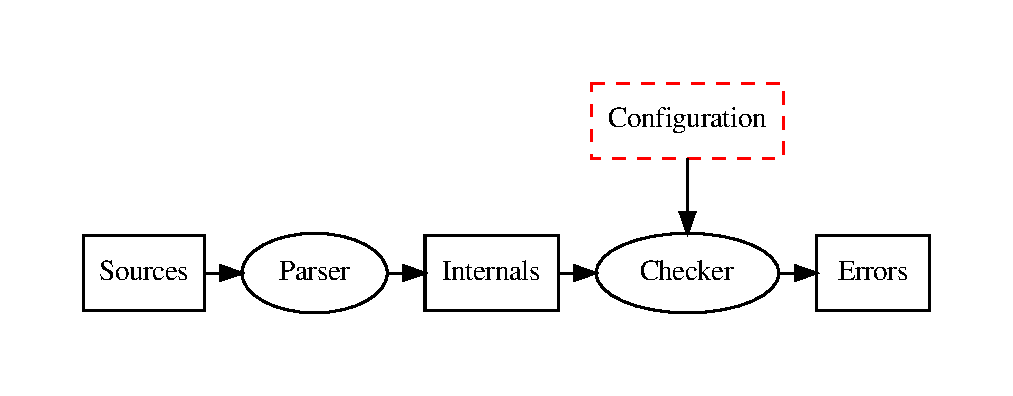
\includegraphics[trim=1.3cm 1.3cm 1.3cm 1.3cm,width=10cm]{level-conf}
  \end{center}

  \begin{itemize}
  \item Checkers can load XML files with configuration
  \item AutomatonChecker -- FA description
  \item ThreadChecker -- thread-creation and locking functions
  \item LockChecker -- locking functions and ratio
  \end{itemize}

\end{frame}

\begin{frame}
  \frametitle{Errors}

  \begin{center}
  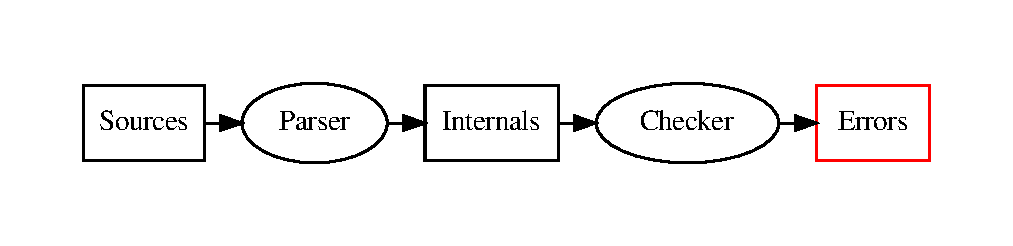
\includegraphics[trim=1.3cm 1.3cm 1.3cm 1.3cm,width=10cm]{level-errors}
  \end{center}

  \heading{Input: Errors from checkers} \\
  \heading{Output: To user}

  \pause
  \medskip

  \begin{itemize}
  \item Command line
  \item Graphical user interface
  \item Web interface
  \end{itemize}

\end{frame}

\begin{frame}
  \frametitle{Found Errors I.}
  
  \heading{ANF Data}
  \begin{itemize}
  \item Missing \texttt{malloc()} return value tests
  \item Memory leaks
  \end{itemize}

  \pause
  \medskip

  \heading{Linux Kernel}\\
  Over 120 errors of the following kinds (reported and fixed):
  \begin{itemize}
  \item Memory errors
  \item Improper locking
    \begin{itemize}
    \item I.e. real deadlocks (cf. example further)
    \end{itemize}
  \item Function pairing
    \begin{itemize}
    \item E.g. get\_cpu/put\_cpu, interrupt enable/disable
    \end{itemize}
  \item (Unintentionally) unreachable code
  \end{itemize}

  \pause
  \medskip

  \heading{Other code}
  \begin{itemize}
  \item SW for CESNET project developing HW accelerators
  \item Small libraries and tools (acl, attr)
  \end{itemize}
\end{frame}

\begin{frame}[fragile]
  \frametitle{Found Errors II.}

  \heading{An example of the Linux kernel bug}

  Source: \texttt{\small linux-2.6.28/drivers/pci/hotplug/pciehp\_core.c}
  \begin{lstlisting}[language=C]
static int set_lock_status(struct hotplug_slot *hotplug_slot,
                           u8 status)
{
  struct slot *slot = hotplug_slot->private;
  ...
  mutex_lock(&slot->ctrl->crit_sect);

  /* has it been >1 sec since our last toggle? */
  if ((get_seconds() - slot->last_emi_toggle) < 1)
    return -EINVAL;
  ...
  mutex_unlock(&slot->ctrl->crit_sect);
  return 0;
}
  \end{lstlisting}

  Trigger: \texttt{\small echo '1' > /sys/bus/pci/slots/.../lock} twice in 1\,s

  \pause
  \medskip

  Full list: \url{http://stanse.fi.muni.cz/bugs.html}

\end{frame}

\begin{frame}
\frametitle{Tools Comparison}
\heading{Many static analysis tools, some of them are compared here}
\small
\begin{tabular}{l|ccccl}
\multirow{2}{*}{Name} &
Open- &
Configu- &
Batch &
Inter- &
\multirow{2}{*}{Languages} \\
%Tool name        & Open & Confi-  & Batch   & Inter- & Languages
                  & source & rable & support & proc.  & \\ \hline
\textsc{\textcolor{red}{Coverity}}$^\dagger$
		  & no   & yes     & yes     & yes    & GC, C++, C\#, Java \\
\textsc{\textcolor{red}{Klocwork}}$^\dagger$
		  & no   & yes     & yes     & yes    & GC, C++, C\#, Java \\
\textsc{Splint}   & yes  & no      & no      & no     & C \\
\textsc{Sparse}   & yes  & no      & yes     & no     & GC \\
\textsc{Clang}    & yes  & no      & yes     & no     & GC, C++, Obj-C \\
\textsc{Uno}      & yes  & yes     & no      & yes    & C$^\dagger$ \\
\textsc{Stanse}   & yes  & yes     & yes     & yes    & GC \\
\textsc{FindBugs} & yes  & no      & yes     & no     & Java \\ \hline
\multicolumn{6}{l}{\footnotesize GC means GNU C} \\
\multicolumn{6}{l}{\footnotesize $^\dagger$\textcolor{red}{Leaders}} \\
\multicolumn{6}{l}{\footnotesize $^\ddagger$Support for C in \textsc{Uno}
does not even contain full C99} \\
\end{tabular}
\end{frame}

\begin{frame}
  \frametitle{Conclusion}
  \begin{itemize}
  \item \textsc{Stanse} is rather a \emph{framework}
  \begin{itemize}
  \item For \emph{easy implementation} of new techniques
  \item But contains also \emph{checkers}
  \end{itemize}
  \item It found \emph{many errors} in real code
  \item More information at \url{http://stanse.fi.muni.cz/}
  \end{itemize}

  \pause
  \medskip

  \heading{Future Work}
  \begin{itemize}
  \item C++ support -- is being plugged-in
  \item Lower false-positives (30-70 \%) -- techniques are known
  \item Speedup parser
  \item Lower memory footprint (mainly XMLs)
  \end{itemize}

\end{frame}

\begin{frame}
  \frametitle{Discussion}
  \begin{center} \huge
  Thanks for your attention! \\[2em]
  Questions?
  \end{center}
\end{frame}

\end{document}

